\chapter{Analisis}
\label{chap: analisis}

\section{Analisis Data Penilaian Skripsi}
\label{sec: analisisData}

	Pada bab ini akan dijelaskan mengenai analisis kode dari sistem kini, analisis tampilan sistem kini, analisis \textit{database} sistem kini, dan analisis sistem usulan.
	
	\subsection{Analisis Kode Sistem Kini}
	\label{sec: analisisKode}
	
		Berdasarkan hasil analisis kode yang telah dibuat, berikut ini adalah penjelasan secara umum mengenai struktur kode Sistem Informasi Penilaian Skripsi 2 Gambar \ref{fig:strukturFile}:
		
		\begin{enumerate}
			\item \textit{Folder} "application" merupakan tempat penyimpanan \textit{Model, View, Controller} dan fungsi-fungsi penting pada \textit{codeigniter}
			\item \textit{Folder} "nbproject" merupakan tempat yang dibutuhkan agar sistem yang tersedia dapat dipakai pada \textit{platform netbeans}. 
			\item \textit{Folder} "public" merupakan tempat penyimpanan \textit{file-file} Javascript dan css yang diperlukan oleh program.
			\item \textit{Folder} "system" merupakan inti dari semua sistem \textit{codeigniter}.
			\item \textit{Folder} "user\_guide" merupakan tempat penyimpanan instruksi-instruksi yang menjadi bantuan bagi pengguna \textit{codeigniter}.
		\end{enumerate}
		
		\begin{figure}[H]
			\centering
			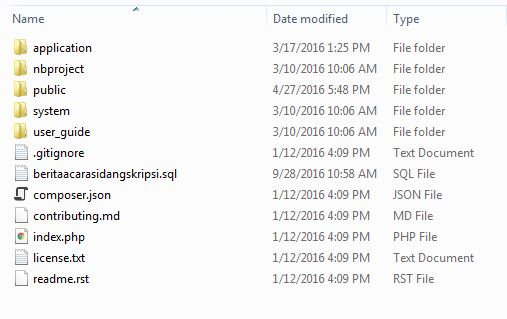
\includegraphics[scale= 1.0]{Gambar/strukturFile}
			\caption {Struktur penyimpanan data program}
			\label{fig:strukturFile}
		\end{figure}
		
		\begin{figure}[H]
			\centering
			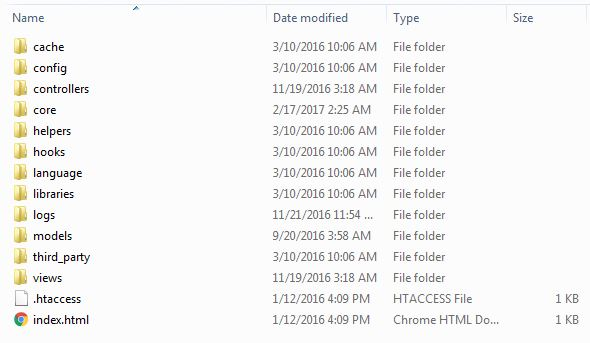
\includegraphics[scale=1.0]{Gambar/strukturFileApp}
			\caption{Struktur file application}
			\label{fig: strukturFileApp}
		\end{figure}
		
		
		Pembuatan sistem informasi penilaian skripsi 2 berfokus pada \textit{folder "application"} (Gambar \ref{fig: strukturFileApp}) yang merupakan tempat penyimpanan \textit{file-file} MVC yang menjadi dasar dari sistem ini.
		
		\begin{enumerate}
			\item \textit{Folder} "config" merupakan tempat penyimpanan \textit{file} yang berguna untuk mengatur berbagai fungsi yang terdapat pada codeigniter.
			\item \textit{Folder} "controller" merupakan tempat penyimpanan \textit{file} yang berfungsi untuk menyambungkan \textit{view} dengan \textit{model} dan mengatur \textit{routing}.
			\item \textit{Folder} "models" merupakan tempat penyimpanan \textit{file model} yang menyambungkan program dengan perintah-perintah sql untuk \textit{database}.
			\item \textit{Folder} "views" merupakan tempat penyimpanan \textit{file-file} yang mengatur tampilan program.
		\end{enumerate}
		
		\begin{figure}[H]
			\centering
			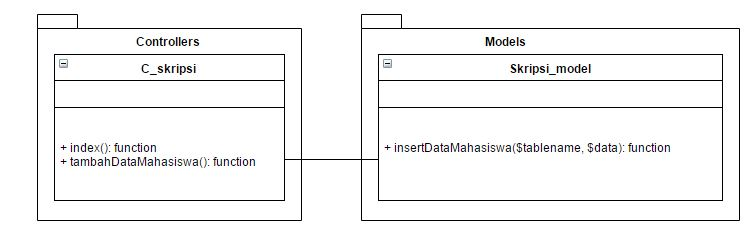
\includegraphics[scale=0.75]{Gambar/diagKelas}
			\caption{Diagram kelas}
			\label{fig: diagramKelas}
		\end{figure}
		
		Berdasarkan diagram kelas dari sistem kini (Gambar \ref{fig: diagramKelas}), maka selanjutnya akan dijelaskan fungsi dari masing-masing metode yang ada:\\
		Kelas C\_Skripsi:
			\begin{itemize}
				\item public function index() \\
				Berfungsi untuk mengarahkan pengguna ke halaman "application/views/"\\
				Nilai kembalian: halaman sistem kini
				\item public function tambahDataMahasiswa() \\
				Berfungsi untuk menerjemahkan \textit{input data} yang telah dimasukkan pengguna pada \textit{view} sehingga dapat diterima oleh \textit{model} sistem kini, yang pada akhirnya akan diproses untuk dimasukkan ke dalam \textit{database} sistem kini.\\
				Nilai kembalian: data yang diperlukan oleh model dalam fungsi insertData.
			\end{itemize}
		Kelas Skripsi\_model:
			\begin{itemize}
				\item public function insertDataMahasiswa(\$tablename, \$data)\\
				Berfungsi untuk memproses \textit{input data} yang sudah diproses oleh \textit{controller} untuk dimasukkan ke dalam \textit{database}\\
				Parameter:\dots{}
					\begin{itemize}
						\item tablename adalah nama tabel.
						\item data adalah kumpulan \textit{input} yang sudah diolah sehingga dapat dimasukkan ke dalam fungsi sql.
					\end{itemize}
			\end{itemize}
		
		\begin{figure}[H]
			\centering
			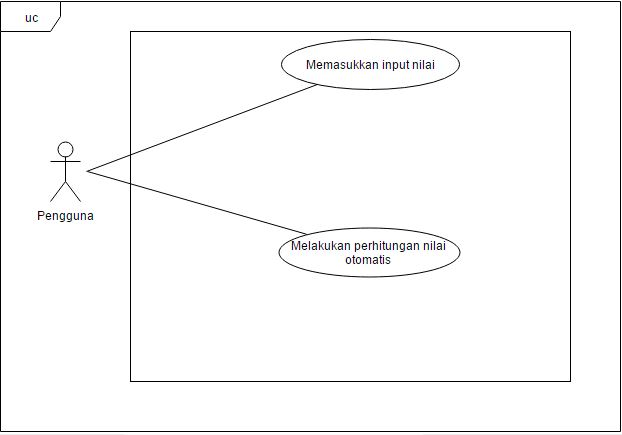
\includegraphics[scale=1.00]{Gambar/usecase}
			\caption{\textit{Use case} diagram}
			\label{fig: usecase}
		\end{figure}
	
		
	\subsection{Analisis Database Sistem Kini}
	\label{sub: analisisDatabase}
	
	Sistem informasi penilaian sidang skripsi 2 menggunakan perangkat lunak phpmyadmin sebagai sarana penyimpanan dan pengolahan \textit{database}. Seperti yang dijelaskan pada subbab \ref{sec: analisisKode}, didalam \textit{folder} "application" terdapat \textit{folder} "models" (Gambar\ref{fig:strukturFileApp}) yang berfungsi menghubungkan \textit{database} dengan sistem. 
	
	Berdasarkan analisa dari contoh form penilaian skripsi yang ada (gambar \ref{fig: skripsiAsli} dan gambar \ref{fig: rekapAsli}), dapat disimpulkan bahwa penilaian skripsi membutuhkan data-data sebagai berikut:
		
		\begin{enumerate}
			\item Semester
			\item Tahun ajaran
			\item NPM mahasiswa 
			\item Nama mahasiswa
			\item Judul skripsi
			\item Nama pembimbing utama/tunggal
			\item Nama pembimbing pendamping(tidak harus)
			\item Nama ketua tim penguji
			\item Nama anggota tim penguji
			\item Bobot ketua tim penguji
			\item Bobot anggota tim penguji
			\item Bobot pembimbing
			\item Nilai koordinator skripsi
			\item Bobot koordinator skripsi
			\item Bobot tata tulis laporan ketua
			\item Bobot kelengkapan materi ketua
			\item Bobot penguasaan materi ketua
			\item Bobot presentasi ketua
			\item Bobot pencapaian tujuan ketua
			\item Bobot tata tulis laporan anggota
			\item Bobot kelengkapan materi anggota
			\item Bobot penguasaan materi anggota
			\item Bobot presentasi anggota
			\item Bobot pencapaian tujuan anggota
			\item Bobot tata tulis laporan pembimbing
			\item Bobot kelengkapan materi pembimbing
			\item Bobot penguasaan materi pembimbing
			\item Bobot bimbingan pembimbing
			\item Nilai akhir mahasiswa
		\end{enumerate}
	
	Berdasarkan diskusi dengan dosen pembimbing, disimpulkan bahwa sistem penilaian sidang skripsi 2 ini hanya memerlukan penyimpanan untuk bobot masing-masing penilaian dan nilai akhir mahasiswa untuk tahap perhitungan. Hal ini dikarenakan nilai-nilai lainnya dapat dihasilkan dengan melakukan perhitungan pada  nilai akhir mahasiswa dan bobot nilai yang diinginkan. Begitu pula dengan nilai dari masing-masing penguji.
	
		\begin{figure}[H]
			\centering
			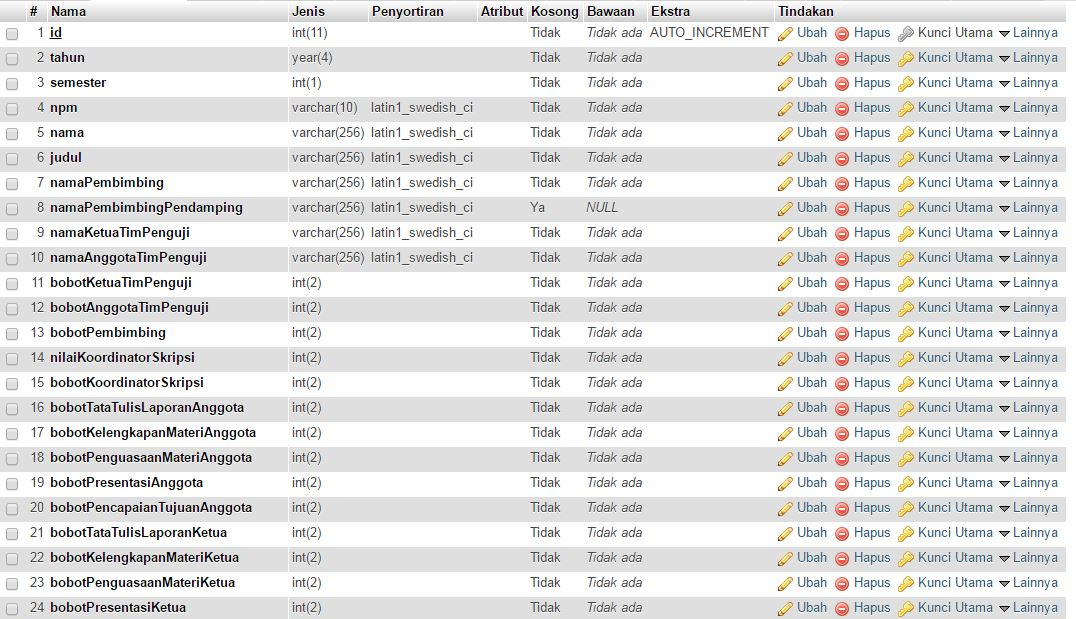
\includegraphics[scale= 1.0]{Gambar/database1}
			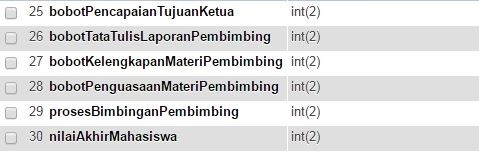
\includegraphics[scale= 1.0]{Gambar/database2}
			\caption {Data yang disimpan di database}
			\label{fig:tabeldata}
		\end{figure}
	
\section{Analisis Tampilan Sistem Informasi Penilaian Skripsi}
\label{sec: analisisTampilan}
	
	Tampilan pada sistem informasi penilaian skripsi haruslah dibuat semirip mungkin dengan form penilaian skripsi yang sudah ada seperti pada lampiran gambar \ref{fig: skripsiAsli} dan gambar \ref{fig: rekapAsli}.
	
	Perbedaan yang akan ditampilkan adalah dengan adanya otomatisasi penghitungan nilai sesuai dengan bobot yang diberikan kepada penilai. Hal ini akan memberikan kemudahan penilai untuk melakukan penilaian.
	
	Gambar \ref{fig:tampilan} adalah bayangan awal tampilan untuk sistem informasi penilaian skripsi:
	\begin{figure}[H]
		\centering
		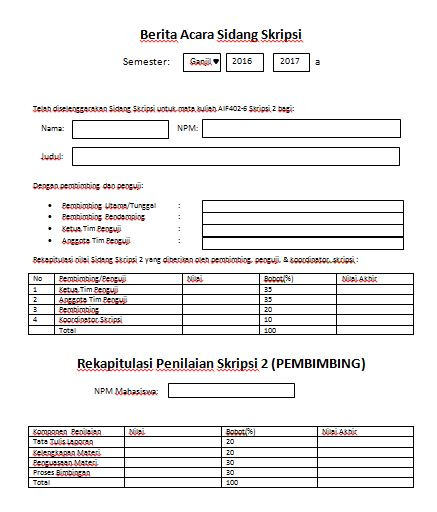
\includegraphics[scale=0.75]{Gambar/tampilan1}
		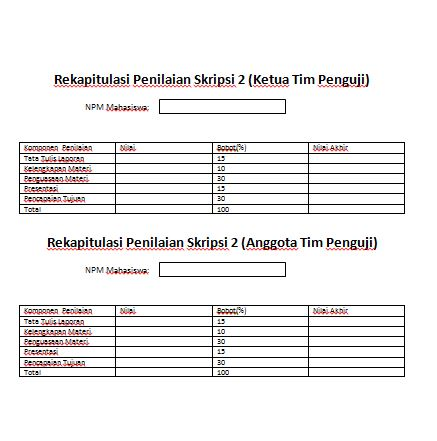
\includegraphics[scale=0.75]{Gambar/tampilan2}
		\caption{Perkiraan Tampilan}
		\label{fig:tampilan}
	\end{figure}
	
	Dari bayangan awal itulah, saya mendesain tampilan dari aplikasi sistem informasi penilaian skripsi 2 ini. Gambar \ref{fig:tampilanapp} merupakan tampilan pada aplikasi sistem informasi penilaian skripsi 2.
	
	\begin{figure}[H]
		\centering
		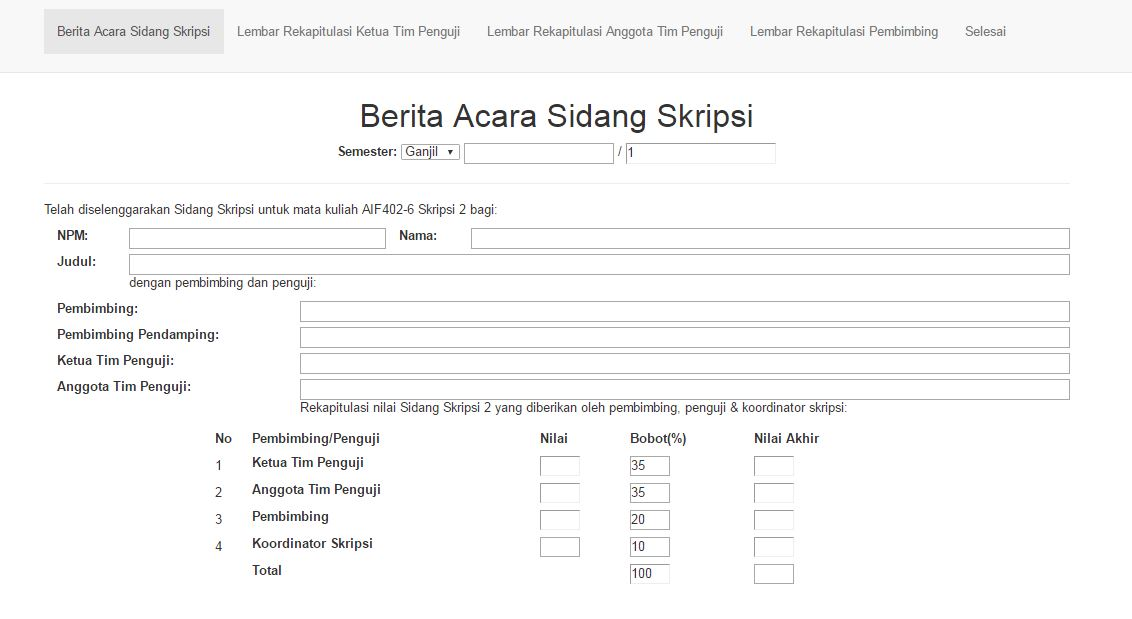
\includegraphics[scale=0.5]{Gambar/tampilanapp1}
		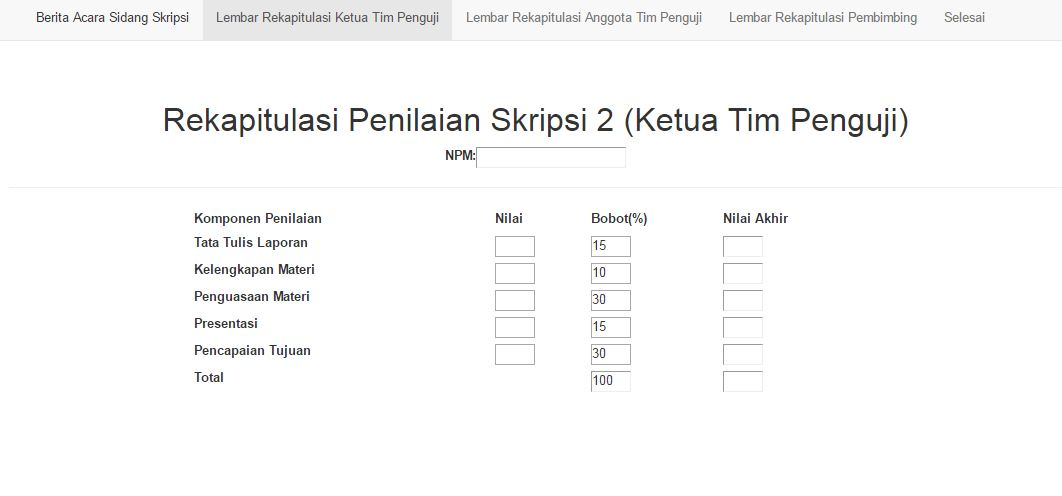
\includegraphics[scale=0.5]{Gambar/tampilanapp2}
		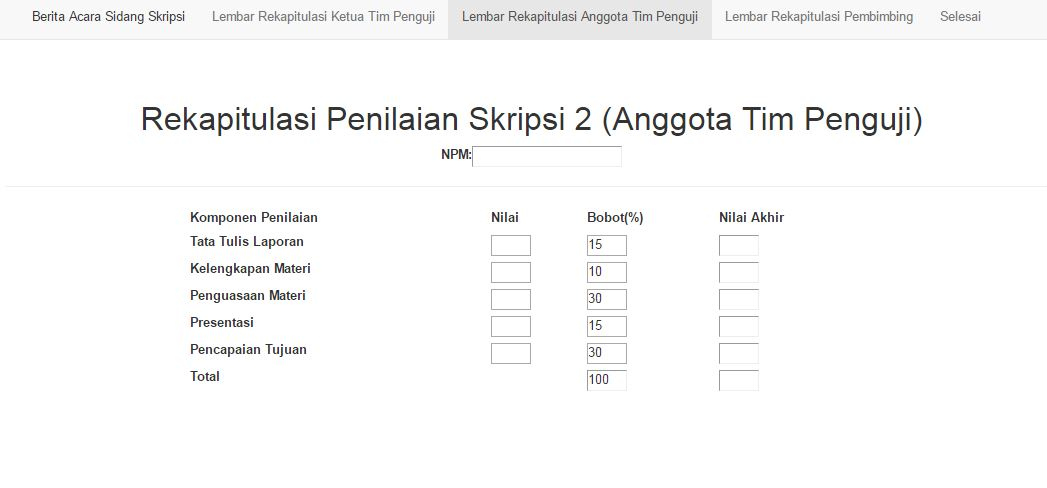
\includegraphics[scale=0.5]{Gambar/tampilanapp3}
		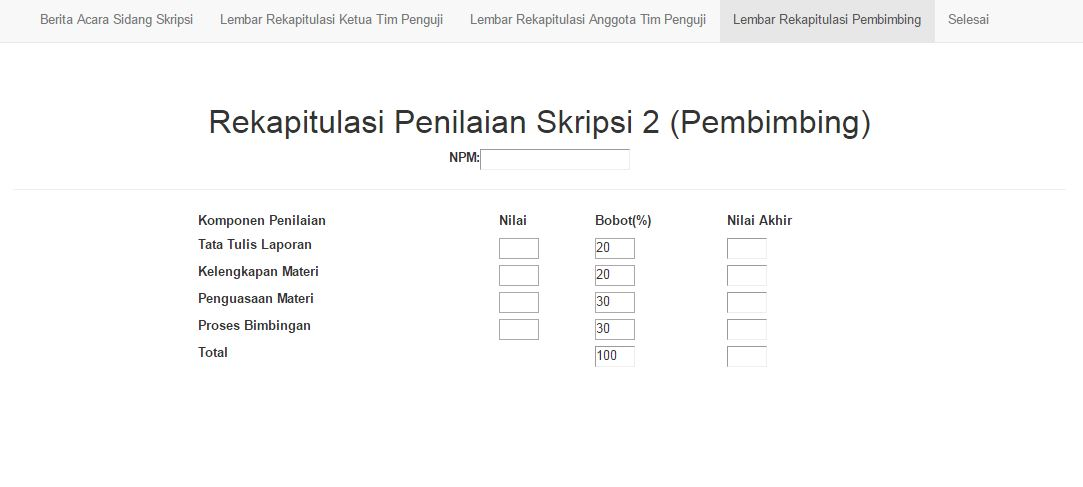
\includegraphics[scale=0.5]{Gambar/tampilanapp4}
		\caption{Perkiraan Tampilan}
		\label{fig:tampilanapp}
	\end{figure}